\documentclass[letterpaper]{article}
\usepackage{amsmath,amssymb}
\usepackage{tikz}
\usepackage[letterpaper,margin=1in]{geometry}
\setlength{\parindent}{0pt}
\newcommand{\noteheader}[1]{\par\medskip\noindent\textbf{#1}\ }

\begin{document}

\textbf{MATH 1564 --- Notes 10/01}

\bigskip

\textbf{Markov chains --- library example}

\medskip

A small town has two libraries, $A$ and $B$.

Each month, among books checked out from library $A$:
\begin{itemize}
\item $80\%$ are returned to $A$;
\item $20\%$ are returned to $B$.
\end{itemize}

Each month, among books checked out from library $B$:
\begin{itemize}
\item $30\%$ are returned to $A$;
\item $70\%$ are returned to $B$.
\end{itemize}

If initially $A$ has 500 books and $B$ has 500 books, how many books will each library have after $k$ months?

\noteheader{Model.} Let
\[
a_k=\text{number of books in $A$ after $k$ months},
\qquad
b_k=\text{number of books in $B$ after $k$ months}.
\]
Then
\[
a_{k+1}=0.8a_k+0.3b_k,
\qquad
b_{k+1}=0.2a_k+0.7b_k.
\]
In matrix form,
\[
X_k=\begin{bmatrix}a_k\\b_k\end{bmatrix},
\qquad
X_{k+1}=\begin{bmatrix}a_{k+1}\\b_{k+1}\end{bmatrix},
\]
and
\[
X_{k+1}=PX_k,
\qquad
P=\begin{bmatrix}0.8&0.3\\0.2&0.7\end{bmatrix}.
\]

\clearpage

Initially,
\[
X_0=\begin{bmatrix}500\\500\end{bmatrix},
\qquad
X_1=PX_0,
\qquad
X_2=PX_1=P^2X_0.
\]

It is better to replace
\[
\begin{bmatrix}a_k\\b_k\end{bmatrix}
\]
by
\[
\frac{1}{1000}\begin{bmatrix}a_k\\b_k\end{bmatrix}.
\]
Then
\[
\frac{a_k}{1000}=\text{the proportion of books in $A$ after $k$ months},
\]
and
\[
\frac{b_k}{1000}=\text{the proportion of books in $B$ after $k$ months}.
\]

\clearpage

\textbf{Definition.} A \textbf{probability vector} is a vector
\[
\begin{bmatrix}x_1\\\vdots\\x_n\end{bmatrix}\in\mathbb{R}^n
\]
such that every $x_i\geq0$ and
\[
x_1+\cdots+x_n=1.
\]
Its coordinates are probabilities of possible outcomes.

\noteheader{Example.} A coin toss has two outcomes, head and tail, represented by the probability vector
\[
\begin{bmatrix}0.5\\0.5\end{bmatrix}.
\]

\bigskip

\noteheader{Definition.} A \textbf{stochastic matrix} is an $n\times n$ matrix whose columns are probability vectors.

\bigskip

\noteheader{Definition.} A \textbf{discrete Markov chain} is a sequence of probability vectors in which each vector is determined by the preceding vector.

\noteheader{Example.} If $X_0$ is a probability vector in $\mathbb{R}^n$ and $P$ is a stochastic matrix, then
\[
X_k=P^kX_0
\]
is a probability vector for every $k$. Therefore, $(X_k)$ is a Markov chain.

\clearpage

\textbf{Theorem.} If $X_0$ is a probability vector and $P$ is stochastic, then
\[
X_k=P^kX_0
\]
is a probability vector for every $k$.

\noteheader{Proof.} Use induction on $k$.

\noteheader{Base case:} For $k=0$, the vector $X_0$ is a probability vector by assumption.

\noteheader{Inductive step:} Suppose $X$ is a probability vector. We show that $PX$ is a probability vector. Write
\[
P=\begin{bmatrix}
a_{11}&\cdots&a_{1n}\\
\vdots&\ddots&\vdots\\
a_{n1}&\cdots&a_{nn}
\end{bmatrix},
\qquad
X=\begin{bmatrix}x_1\\\vdots\\x_n\end{bmatrix}.
\]
Then
\[
PX=\begin{bmatrix}
a_{11}x_1+\cdots+a_{1n}x_n\\
\vdots\\
a_{n1}x_1+\cdots+a_{nn}x_n
\end{bmatrix}.
\]
Every entry of $PX$ is nonnegative because the entries of $P$ and $X$ are nonnegative. The sum of the entries of $PX$ is
\[
(a_{11}+\cdots+a_{n1})x_1+\cdots+(a_{1n}+\cdots+a_{nn})x_n.
\]

\clearpage

Because each column of $P$ is a probability vector,
\[
a_{1j}+\cdots+a_{nj}=1
\quad\text{for each }j.
\]
Therefore,
\[
(a_{11}+\cdots+a_{n1})x_1+\cdots+(a_{1n}+\cdots+a_{nn})x_n
=x_1+\cdots+x_n=1.
\]
Thus $PX$ is a probability vector.

\bigskip

\noteheader{Conclusion.} The recursion
\[
X_{k+1}=PX_k
\]
models a change in outcome probabilities from time $k$ to time $k+1$.

\noteheader{Example.}
\[
P=\begin{bmatrix}0.8&0.3\\0.2&0.7\end{bmatrix}
\]
is stochastic, and
\[
X_0=\begin{bmatrix}0.5\\0.5\end{bmatrix}
\]
is a probability vector. Then
\[
X_1=
\begin{bmatrix}0.4+0.15\\0.1+0.35\end{bmatrix}
=\begin{bmatrix}0.55\\0.45\end{bmatrix}.
\]

\bigskip

\noteheader{Definition.} A \textbf{steady state} for $X_{k+1}=PX_k$ is a probability vector $q$ satisfying
\[
Pq=q.
\]

\clearpage

\textbf{Example: steady state for the library model.}
\[
P=\begin{bmatrix}0.8&0.3\\0.2&0.7\end{bmatrix}.
\]
Let
\[
q=\begin{bmatrix}x\\y\end{bmatrix}.
\]
The equation $Pq=q$ is equivalent to
\[
(P-I)q=0,
\]
so
\[
\begin{bmatrix}0\\0\end{bmatrix}
=\begin{bmatrix}-0.2&0.3\\0.2&-0.3\end{bmatrix}
\begin{bmatrix}x\\y\end{bmatrix}
=\begin{bmatrix}-0.2x+0.3y\\0.2x-0.3y\end{bmatrix}.
\]
Thus $2x=3y$. Since $x+y=1$,
\[
x=\frac35,
\qquad y=\frac25,
\qquad q=\begin{bmatrix}3/5\\2/5\end{bmatrix}.
\]

\clearpage

\textbf{Examples: describing steady states}

\begin{enumerate}
\item If
\[
P=\begin{bmatrix}1&0\\0&1\end{bmatrix},
\]
then $Pq=q$ for every probability vector $q$. Thus every probability vector is a steady state.

\item If
\[
P=\begin{bmatrix}0&1\\1&0\end{bmatrix},
\]
then
\[
(P-I)q=
\begin{bmatrix}-1&1\\1&-1\end{bmatrix}q=0.
\]
Hence $q_1=q_2$, and the steady state is
\[
q=\begin{bmatrix}0.5\\0.5\end{bmatrix}.
\]

\item If
\[
P=\begin{bmatrix}1&1\\0&0\end{bmatrix},
\]
then
\[
(P-I)q=
\begin{bmatrix}0&1\\0&-1\end{bmatrix}
\begin{bmatrix}x\\y\end{bmatrix}
=\begin{bmatrix}y\\-y\end{bmatrix}=0.
\]
Thus $y=0$, so the steady state is
\[
q=\begin{bmatrix}1\\0\end{bmatrix}.
\]
\end{enumerate}

\clearpage

\textbf{Theorem.} Every stochastic matrix has a steady state.

\noteheader{Proof for $2\times2$ matrices.} Write
\[
P=\begin{bmatrix}r&1-s\\1-r&s\end{bmatrix},
\qquad 0\leq r,s\leq1.
\]
Then
\[
P-I=
\begin{bmatrix}r-1&1-s\\1-r&s-1\end{bmatrix}.
\]
For $q=\begin{bmatrix}x\\y\end{bmatrix}$, the equation $(P-I)q=0$ is
\[
(r-1)x+(1-s)y=0,
\qquad x+y=1.
\]
If $r+s\ne2$, this gives
\[
q=
\begin{bmatrix}
\dfrac{1-s}{2-r-s}\\[6pt]
\dfrac{1-r}{2-r-s}
\end{bmatrix}.
\]
If $r+s=2$, then $r=s=1$, so $P=I$ and every probability vector is a steady state.

\clearpage

\textbf{Definition.} A stochastic matrix $P$ is \textbf{regular} if $P^k$ has strictly positive entries for some positive integer $k$.

\noteheader{Example.} Is
\[
P=\begin{bmatrix}0&1\\1&0\end{bmatrix}
\]
regular? No, because
\[
P^{2j}=I,
\qquad
P^{2j+1}=P,
\]
so every power has a zero entry.

\noteheader{Example.} Is
\[
P=\begin{bmatrix}1&0.5\\0&0.5\end{bmatrix}
\]
regular? No. Every power of an upper-triangular matrix is upper triangular, so the lower-left entry remains zero.

\clearpage

\noteheader{Example.} Let
\[
P=\begin{bmatrix}
0.5&0.3&0.4\\
0.5&0.3&0.1\\
0&0.4&0.5
\end{bmatrix}.
\]
Then
\[
P^2=
\begin{bmatrix}
0.4&0.4&0.43\\
0.4&0.28&0.28\\
0.2&0.32&0.29
\end{bmatrix},
\]
whose entries are all positive. Therefore, $P$ is regular.

\bigskip

\noteheader{Definition.} A steady state $q$ for a stochastic matrix $P$ is a \textbf{sink} if, for every probability vector $X_0$, the sequence defined by
\[
X_{k+1}=PX_k
\]
converges to $q$.

\noteheader{Example.} If $P$ has a sink $q$, then $q$ is the only steady state of $P$. Indeed, if $q_1$ is another steady state, then $P^kq_1=q_1$ for every $k$; convergence to $q$ forces $q_1=q$.

\noteheader{Example.} Does
\[
P=\begin{bmatrix}0&1\\1&0\end{bmatrix}
\]
have a sink? No. With
\[
X_0=\begin{bmatrix}1\\0\end{bmatrix},
\qquad
q=\begin{bmatrix}0.5\\0.5\end{bmatrix},
\]
the vectors $P^kX_0$ oscillate.

\clearpage

\textbf{Theorem.} Every regular stochastic matrix $P$ has a sink $q$ such that, for every probability vector $X_0$,
\[
\lim_{k\to\infty}P^kX_0=q.
\]

\bigskip

\noteheader{Determinants}

\medskip

For a $2\times2$ matrix,
\[
\det\begin{bmatrix}a&b\\c&d\end{bmatrix}=ad-bc.
\]
For a $1\times1$ matrix,
\[
\det[a]=a.
\]

\noteheader{Motivation.}
\begin{enumerate}
\item $\det:M_{n\times n}(\mathbb{R})\to\mathbb{R}$.
\item The determinant is easily computable.
\item $\det(AB)=\det(A)\det(B)$.
\item $\det A=0$ if and only if $A$ is not invertible (equivalently, $A$ is singular).
\item $|\det[v_1\ \cdots\ v_n]|$ is the volume of the parallelepiped spanned by $v_1,\ldots,v_n$.
\end{enumerate}

\begin{center}
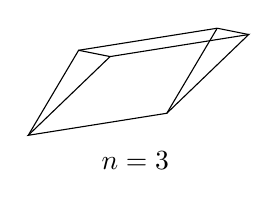
\begin{tikzpicture}[scale=0.8]
\draw (0,0) -- (2.2,0.35) -- (3.5,1.6) -- (1.3,1.25) -- cycle;
\draw (0,0) -- (0.8,1.35) -- (3,1.7);
\draw (0.8,1.35) -- (1.3,1.25);
\draw (2.2,0.35) -- (3,1.7);
\draw (3.5,1.6) -- (3,1.7);
\node at (1.7,-0.4) {$n=3$};
\end{tikzpicture}
\end{center}

\clearpage

\textbf{Definition: cofactor expansion along row one.} If $A=(a_{ij})$ is $n\times n$, then
\[
\det(A)=a_{11}C_{11}+\cdots+a_{1n}C_{1n},
\]
where
\[
C_{1j}=(-1)^{1+j}\det(A_{1j}),
\]
and $A_{1j}$ is the matrix obtained from $A$ by removing row $1$ and column $j$.

\noteheader{Example.}
\begin{align*}
\det\begin{bmatrix}a&b\\c&d\end{bmatrix}
&=aC_{11}+bC_{12}\\
&=a\det[d]+b\bigl(-\det[c]\bigr)\\
&=ad-bc.
\end{align*}

\noteheader{Example.}
\begin{align*}
\det\begin{bmatrix}1&2&-1\\3&1&2\\-1&0&1\end{bmatrix}
&=\det\begin{bmatrix}1&2\\0&1\end{bmatrix}
-2\det\begin{bmatrix}3&2\\-1&1\end{bmatrix}
-\det\begin{bmatrix}3&1\\-1&0\end{bmatrix}\\
&=1-2(3+2)-1\\
&=-10.
\end{align*}

\clearpage

\textbf{Example.} If $A$ is upper triangular, then repeated cofactor expansion along the first row gives
\[
\det(A)=a_{11}a_{22}\cdots a_{nn}.
\]

\bigskip

\noteheader{Change in $\det A$ under row operations}

\noteheader{Rules.}
\begin{enumerate}
\item If $B$ is obtained from $A$ by swapping two rows, then
\[
\det B=-\det A.
\]
For a $2\times2$ matrix,
\[
\det\begin{bmatrix}a&b\\c&d\end{bmatrix}=ad-bc,
\qquad
\det\begin{bmatrix}c&d\\a&b\end{bmatrix}=cb-ad.
\]

\item If $B$ is obtained from $A$ by scaling one row by a constant $c$, then
\[
\det B=c\det A.
\]
\end{enumerate}

\clearpage

\textbf{Intuitive check for row scaling.}
\begin{align*}
\det\begin{bmatrix}a&b\\2c&2d\end{bmatrix}
&=-\det\begin{bmatrix}2c&2d\\a&b\end{bmatrix}\\
&=-2\det\begin{bmatrix}c&d\\a&b\end{bmatrix}\\
&=2\det\begin{bmatrix}a&b\\c&d\end{bmatrix}.
\end{align*}

\noteheader{Rule 3.} Replacing a row by itself plus a multiple of another row does not change the determinant.

\noteheader{Intuitive check.}
\begin{align*}
\det\begin{bmatrix}a&b\\c&d\end{bmatrix}
&=ad-bc,\\
\det\begin{bmatrix}a&b\\2a+c&3b+d\end{bmatrix}
&=a(3b+d)-b(2a+c)\\
&=ad-bc.
\end{align*}

\end{document}
